\begin{frame}
    \frametitle{Abstract}
    \begin{abstract}
    Text-based games, also called text adventures or interactive
    fiction, are a form of games meant to evoke reading a work of
    fiction, where the player controls the main character, popularized
    in the 1980s by games like Zork I\cite{blank_zork_1980}. Players
    interact with the environment through text commands and the game
    gives feedback in the form of natural language descriptions. I
    developed the beginnings of a knowledge and logic-based agent to
    leverage logical reasoning in solving rudimentary text-based games.
\end{abstract}

\end{frame}

\section{Description}

\begin{frame}
    \frametitle{Goal: An AI agent for text-based games}
    \framesubtitle{Design priorities}
    \begin{itemize}
        \item Favor interpretable processes wherever possible
        \item Make inferences about objects in game world based on
            knowledge
        \item Generalize observations between games to make better
            inferences
    \end{itemize}
\end{frame}

\begin{frame}

    \frametitle{What is a text-based game?}
    \begin{columns}
    % timeline of popular games
        \column{.5\textwidth}
        \begin{block}{Popular games}
            {\footnotesize
            \begin{itemize}
                \item \game{Adventure}, William Crowther and Donald
                    Woods, 1976.
                \item \game{Zork I}, Mark Blank and Dave Lebling, 1980.
                \item \game{Enchanted}, Mark Blank and Dave Lebling,
                    1983.
                \item \game{The Hitchiker's Guide to the Galaxy},
                    Douglas Adams and Steve Meretsky, 1984.
                \item \game{Curses}, Graham Nelson, 1993.
                \item \game{Spider and Web}, Andrew Plotkin, 1998.
                \item \game{Counterfeit Monkey}, Emily Short, 2012.
            \end{itemize}
            \parencite{interactive_fiction_technology_foundation_interactive_nodate}
        }
        \end{block}

        % characteristics of games
        \column{.5\textwidth}
        \begin{block}{Common characteristics}
            \begin{itemize}
                \item Players take on the role of a character in an
                    immersive world
                \item A goal, or \emph{quest} is usually given at the
                    start of the game
                \item Players interact with the world by issuing natural
                    language commands
                \item Information about the world is conveyed to the
                    player through prose descriptions
            \end{itemize}
        \end{block}
    \end{columns}

\end{frame}

\begin{frame}[b]
    \begin{figure}
        \centering
        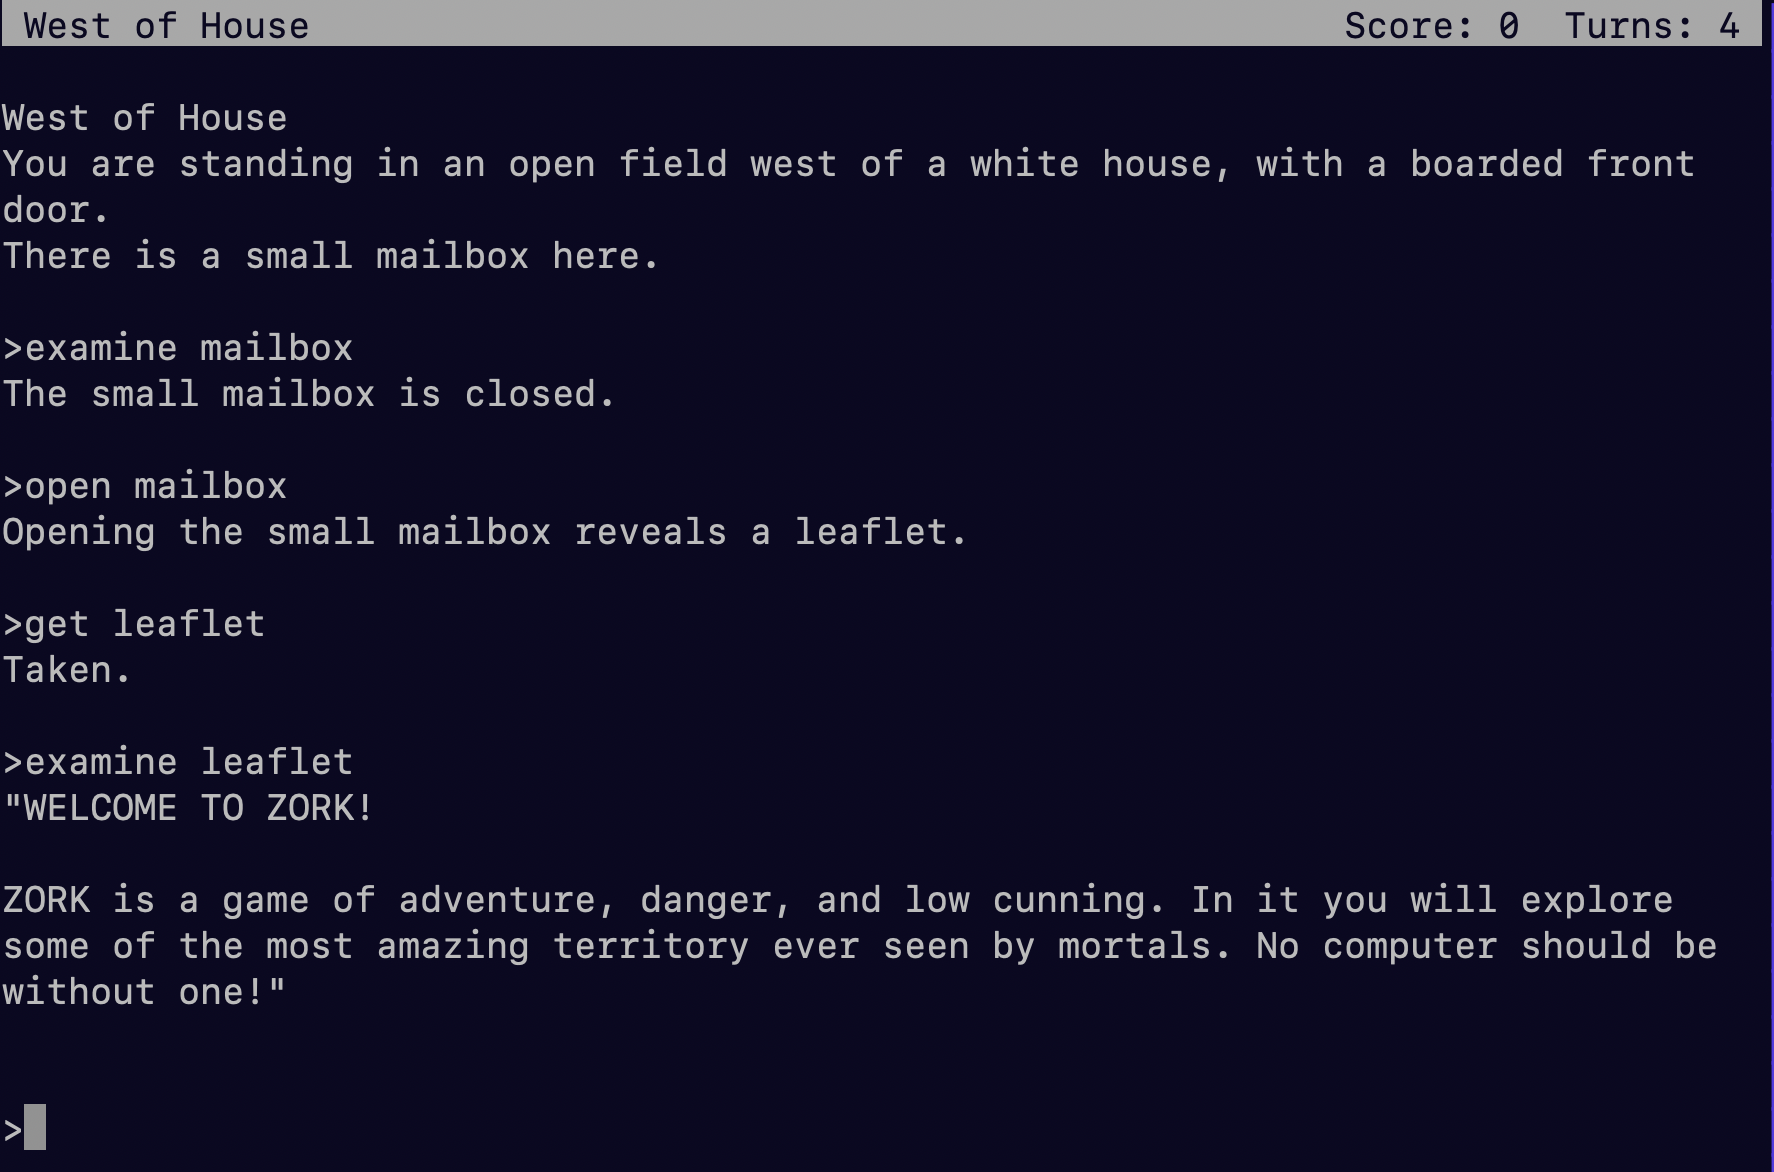
\includegraphics[width=\textwidth,keepaspectratio]{../images/zork1.png}
        \caption*{Zork I, Marc Blank and Dave Lebling, 1980}
    \end{figure}
\end{frame}

\begin{frame}[b]
    \begin{figure}
        \centering
        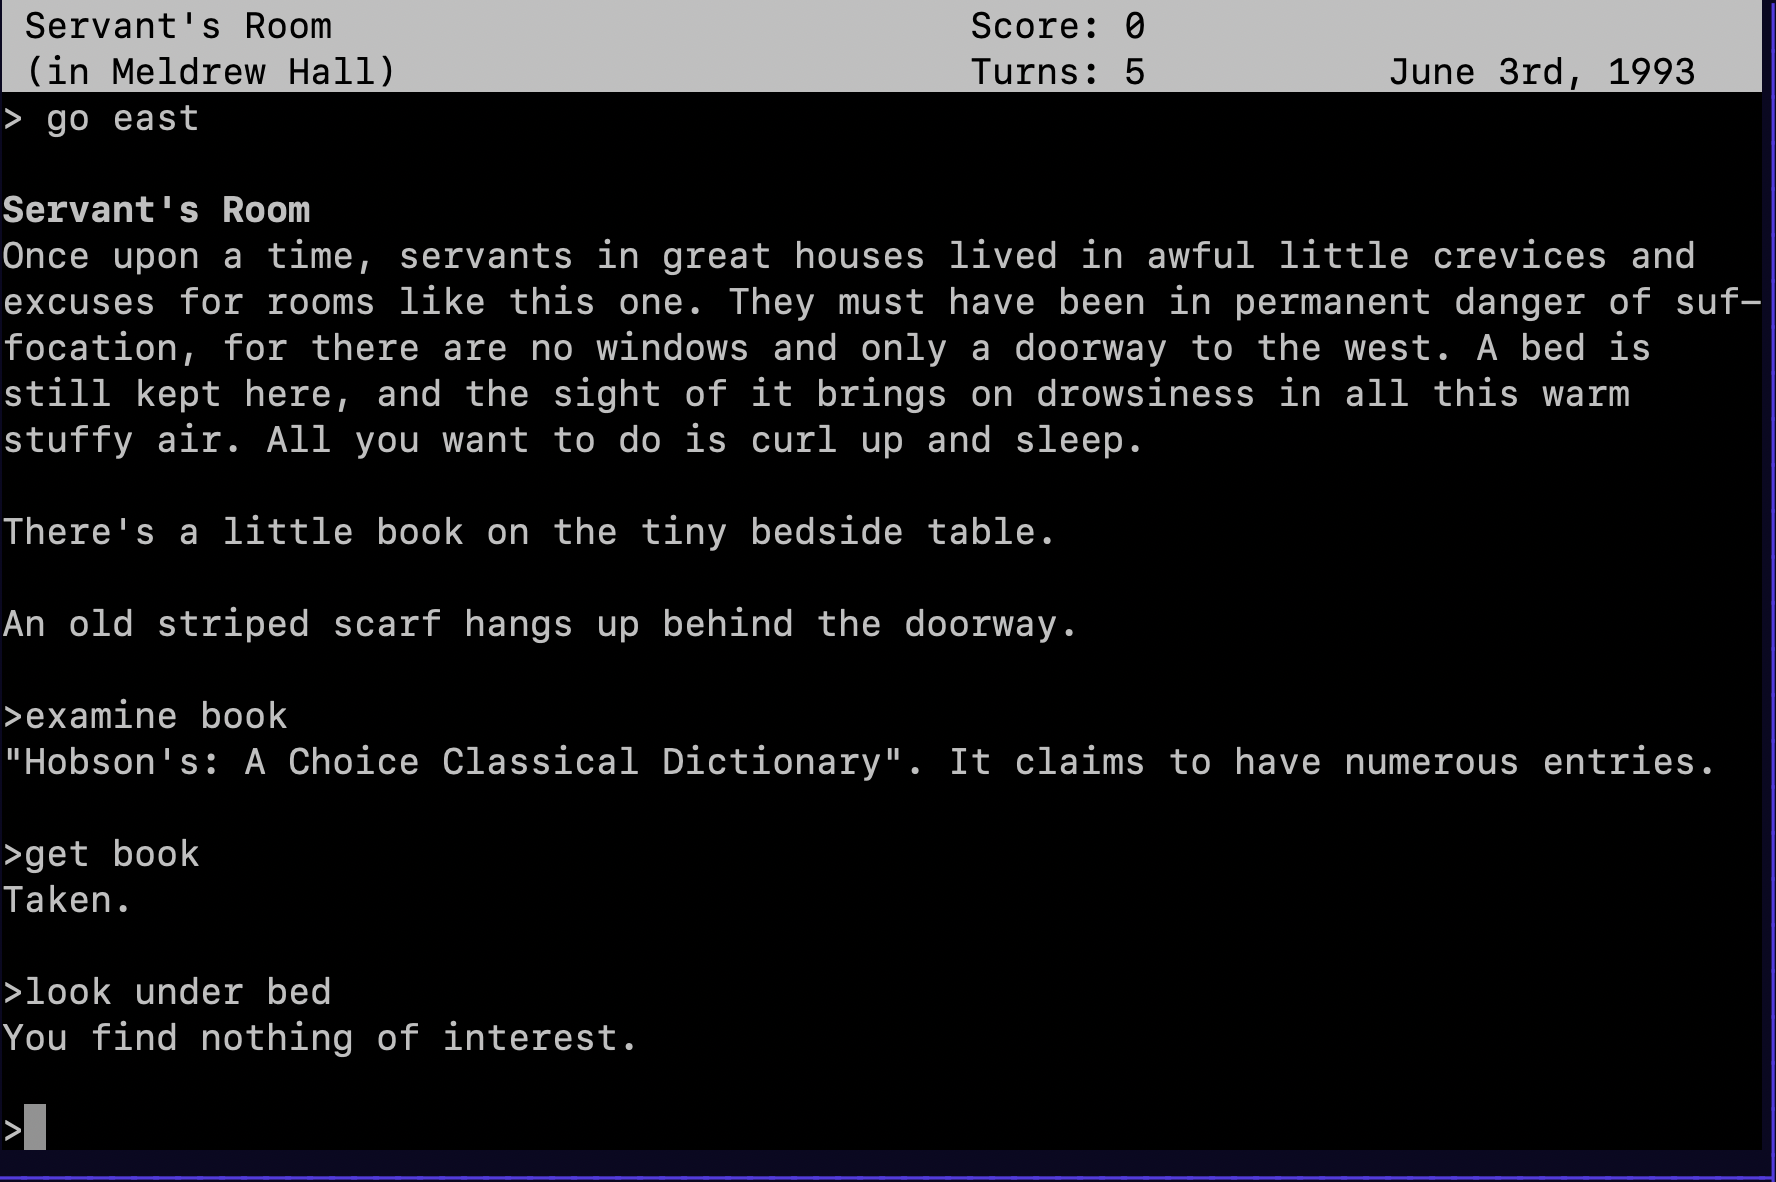
\includegraphics[width=\textwidth,keepaspectratio]{../images/curses.png}
        \caption*{Curses, Graham Nelson, 1993}
    \end{figure}
\end{frame}

\begin{frame}[b]
    \begin{figure}
        \centering
        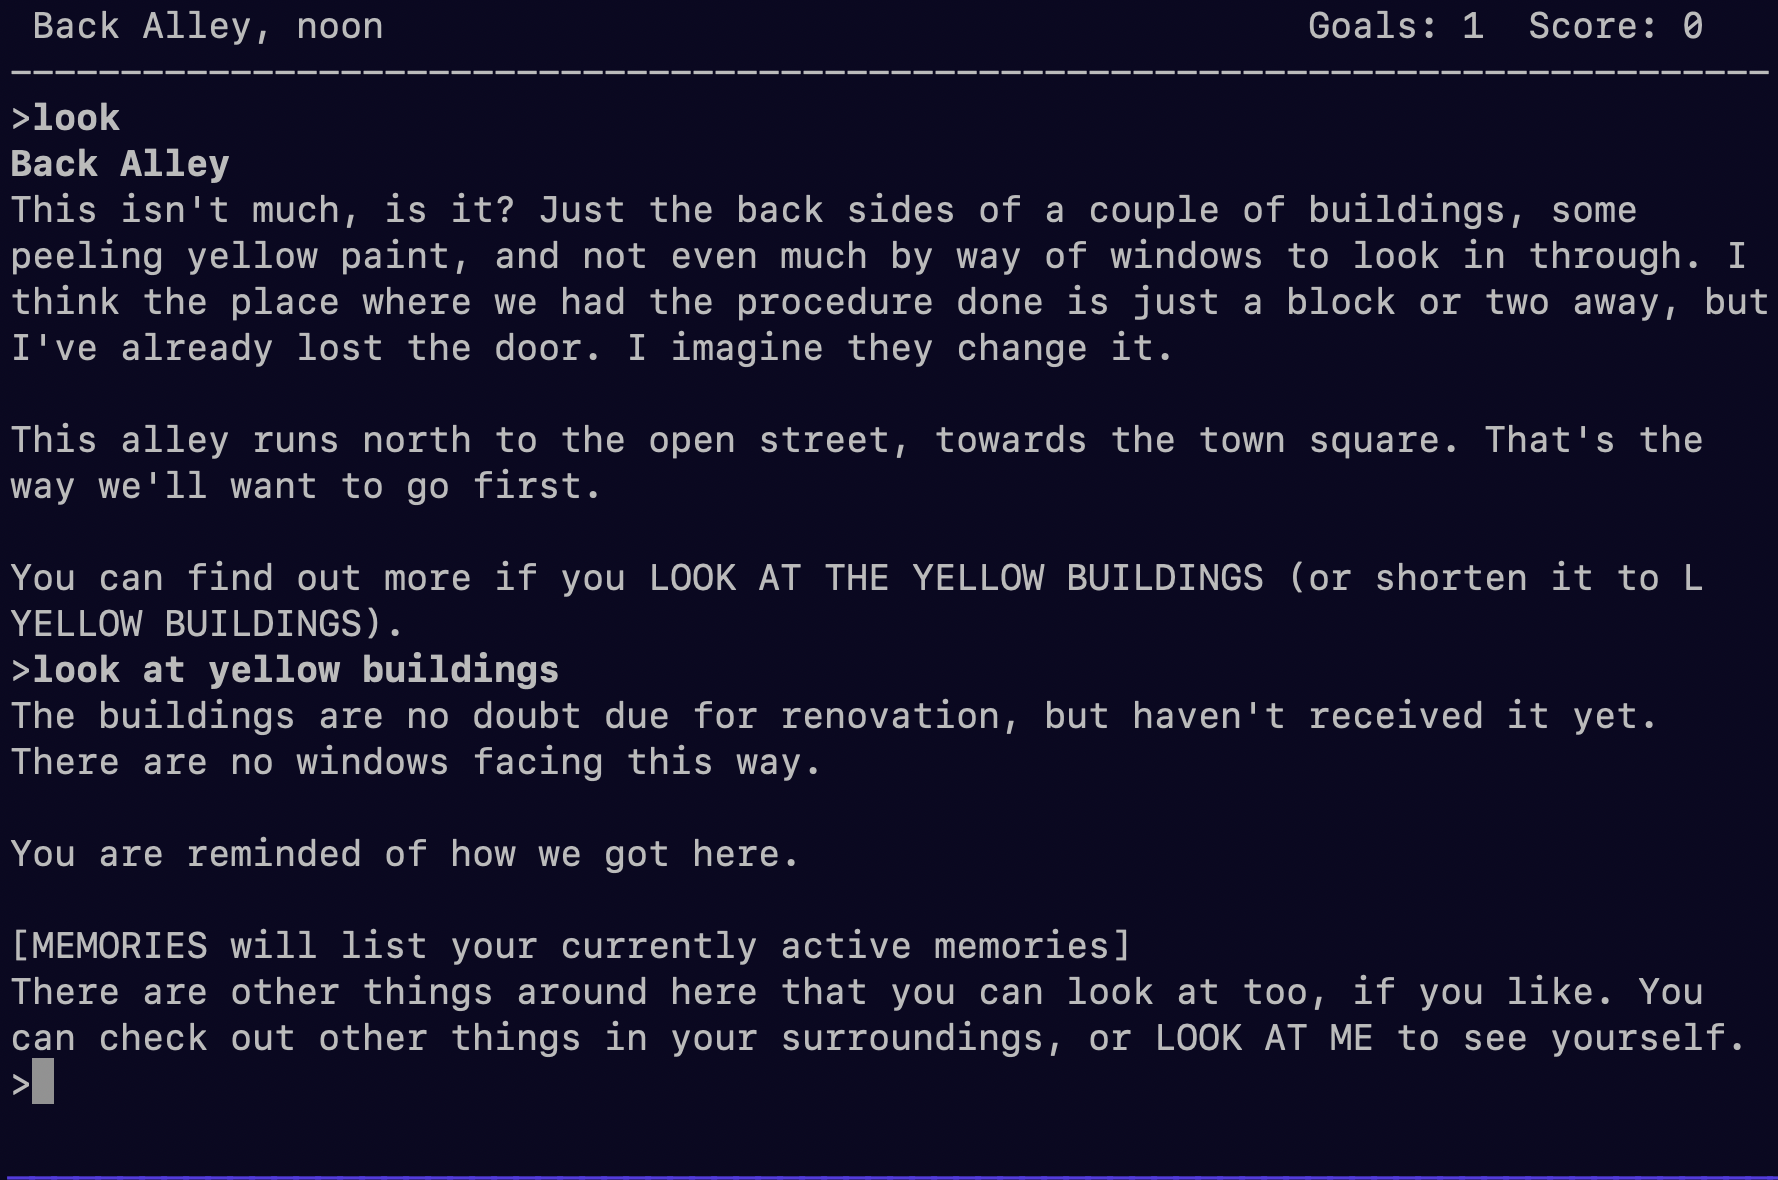
\includegraphics[width=\textwidth,keepaspectratio]{../images/counterfeit_monkey.png}
        \caption*{Counterfeit Monkey, Emily Short, 2012}
    \end{figure}
\end{frame}

\begin{frame}

    \frametitle{Benchmarks}

    Traditional text adventures remain largely unsolvable by AI agents,
    but constrained benchmark games can be created that allow agents to
    focus on specific skills.

    \begin{block}{Evaluation: Solve increasingly complex mazes}
        \begin{enumerate}
            \item Trivial mazes (interconnected areas without obstacles) 
            \item Simple obstacles such as doors
            \item Composite obstacles such as locked doors
            \item Stretch goal: complex, novel obstacles
        \end{enumerate}

    \end{block}

\end{frame}
